\subsection{Mobility}
In \label{fig
}, we conducted a comprehensive simulation of pedestrian flow, modeling the movement patterns of millions of pedestrians who traverse the city's streets in a random manner. The primary objective of this simulation is to identify areas within the urban layout that inherently lead to higher pedestrian densities due to their design. By simulating random pedestrian movements, we can isolate and analyze the impact of urban design on crowding, independent of known hotspots or attractions that typically draw crowds. This approach ensures that the analysis focuses solely on the structural aspects of the city's design, providing insights that can be used to mitigate potential congestion and enhance pedestrian flow through more informed urban planning.
\subsubsection{Pedestrian Flow}
\begin{figure}
    \centering
    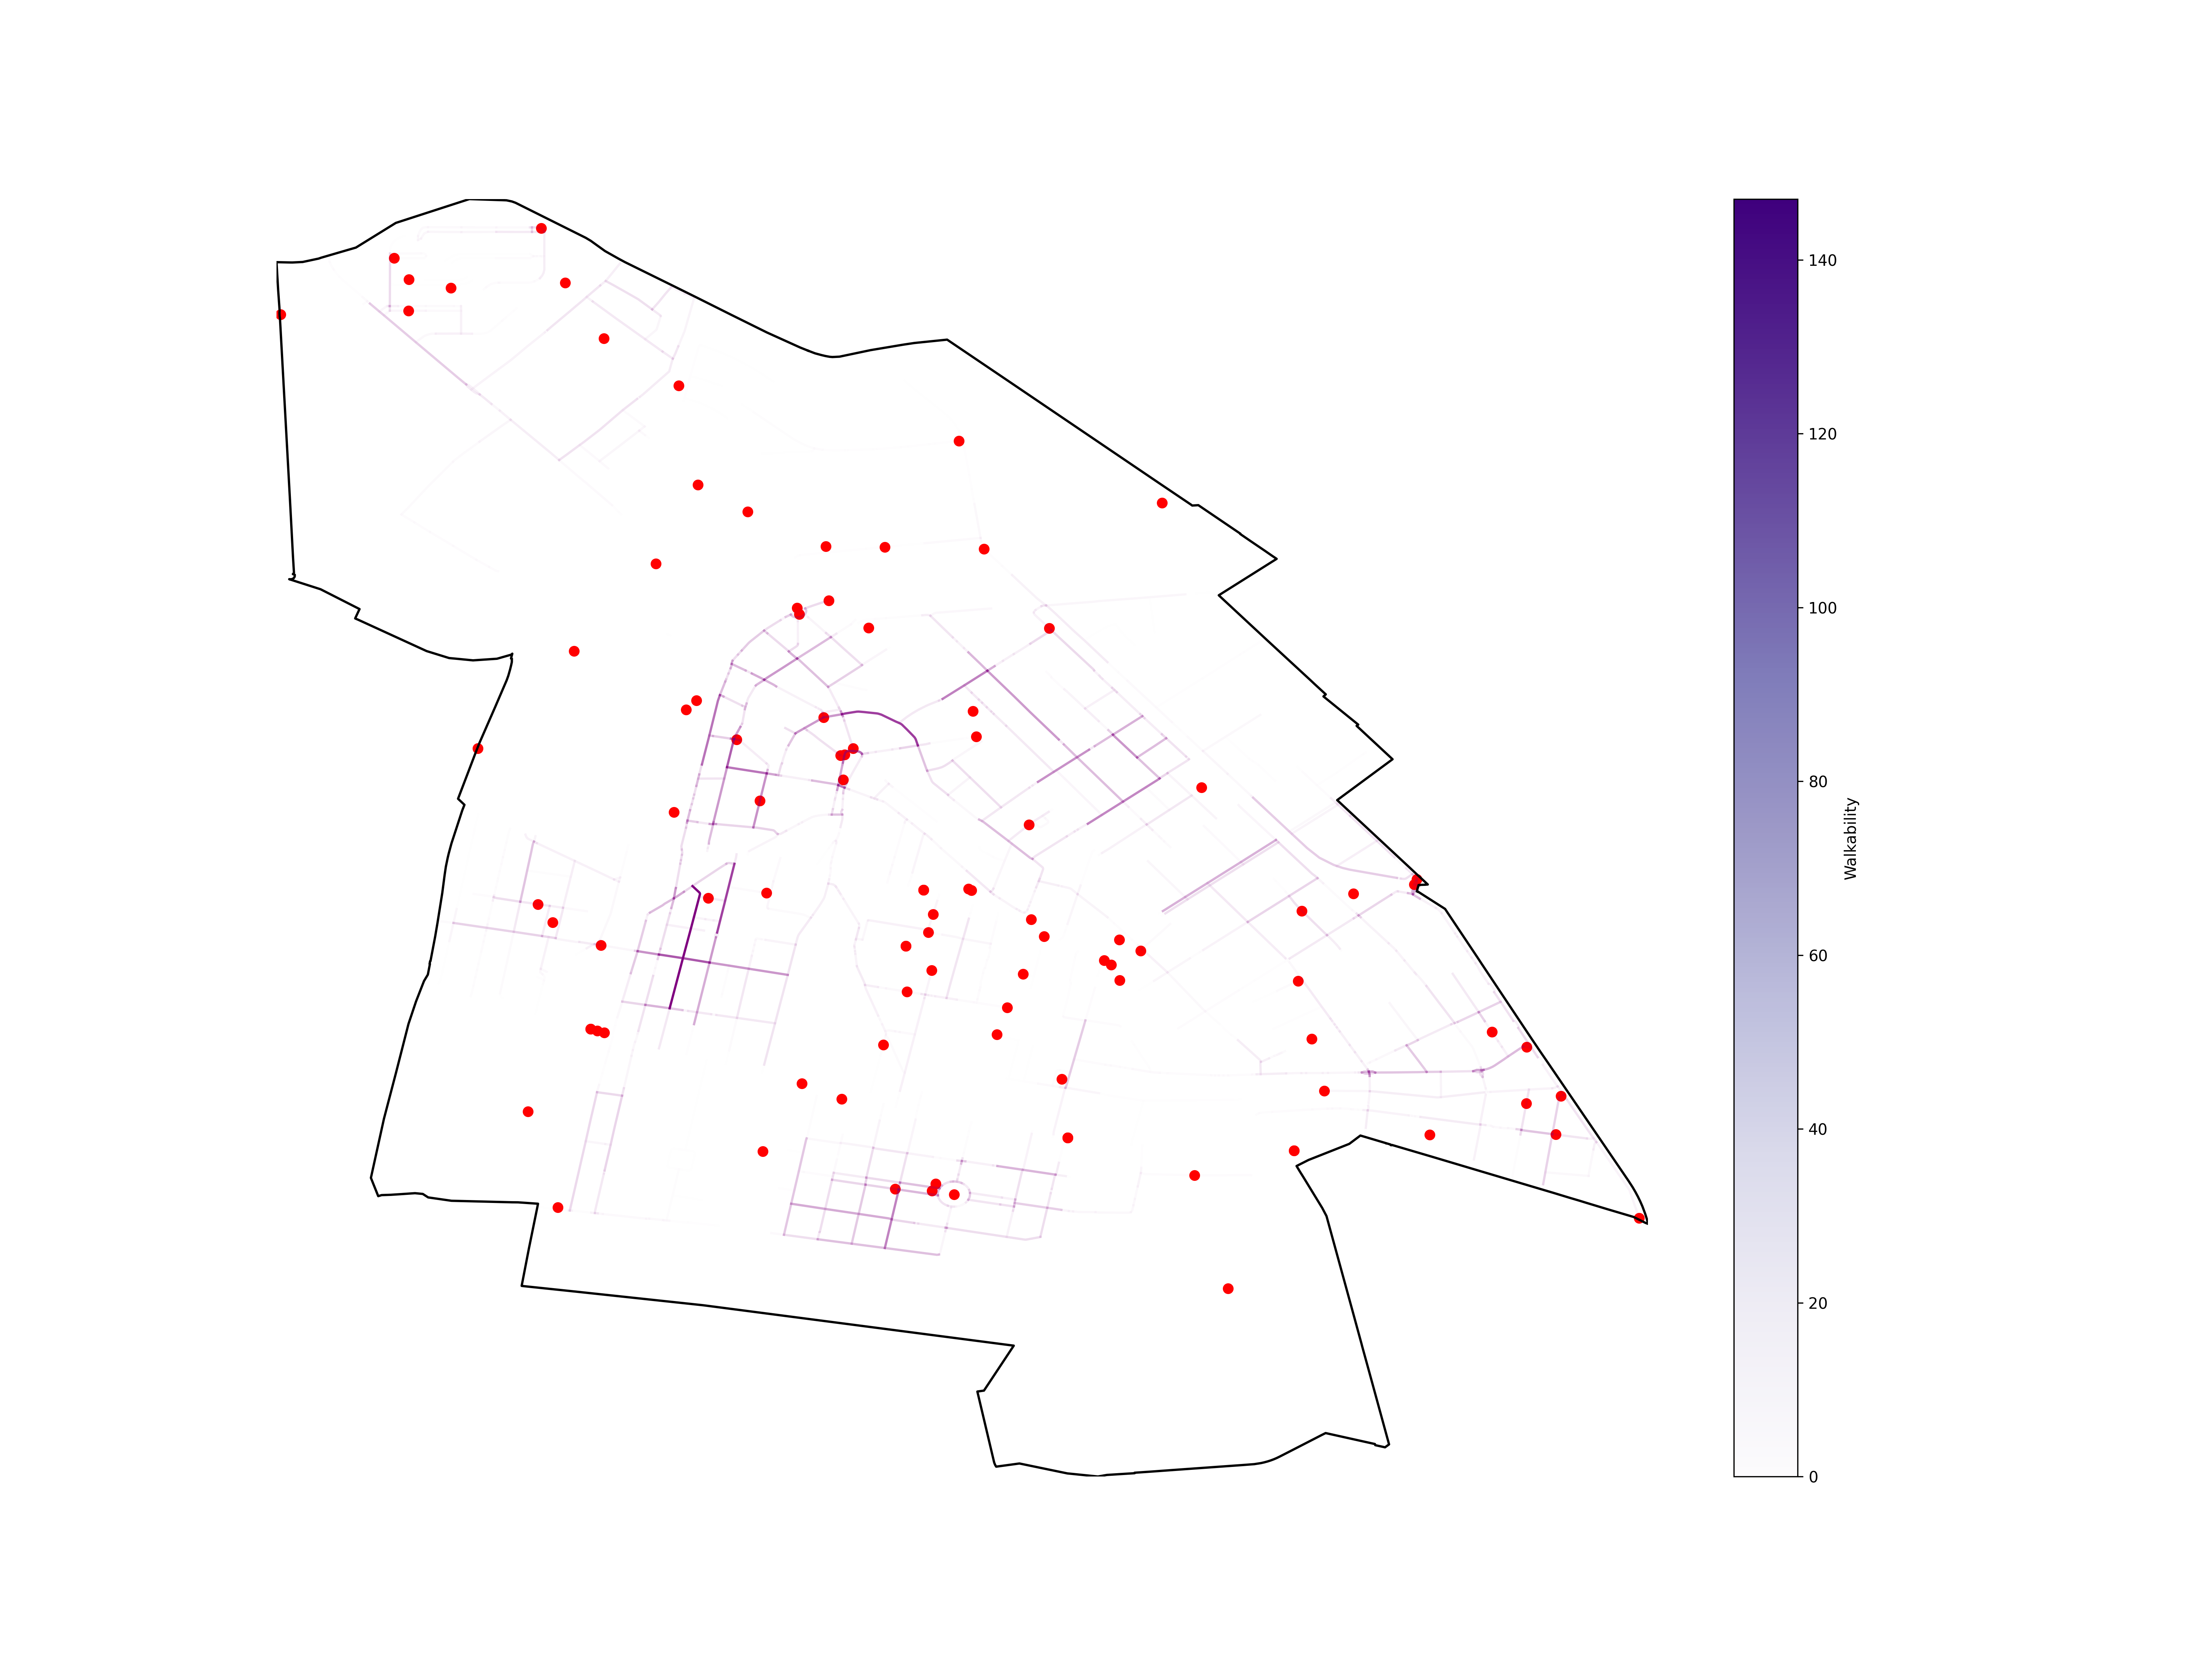
\includegraphics[width=0.7\textwidth]{figures/Adri/random_walk.png}
    \caption{Simulation of pedestrian flow in the city. Darker regions indicate areas with higher pedestrian density, highlighting zones that are prone to crowding due to the city's design.}
    \label{fig:simulation_flow}
\end{figure}
\subsubsection{Street Centralities}

In urban planning and analysis, various graph centrality measures are utilized to assess the importance and connectivity of streets within a city's layout. Each centrality measure provides unique insights into different aspects of the street network, aiding in the identification of critical routes, accessibility, and influential areas. The following visualizations (Figure \ref{fig:centralities}) illustrate the application of four centrality metrics—Betweenness Centrality, Closeness Centrality, Degree Centrality, and PageRank—on a city's street network. These visualizations help urban planners to make informed decisions regarding infrastructure development, traffic management, and urban design improvements.

\begin{figure}
    \centering
    \begin{tabular}{cc}
         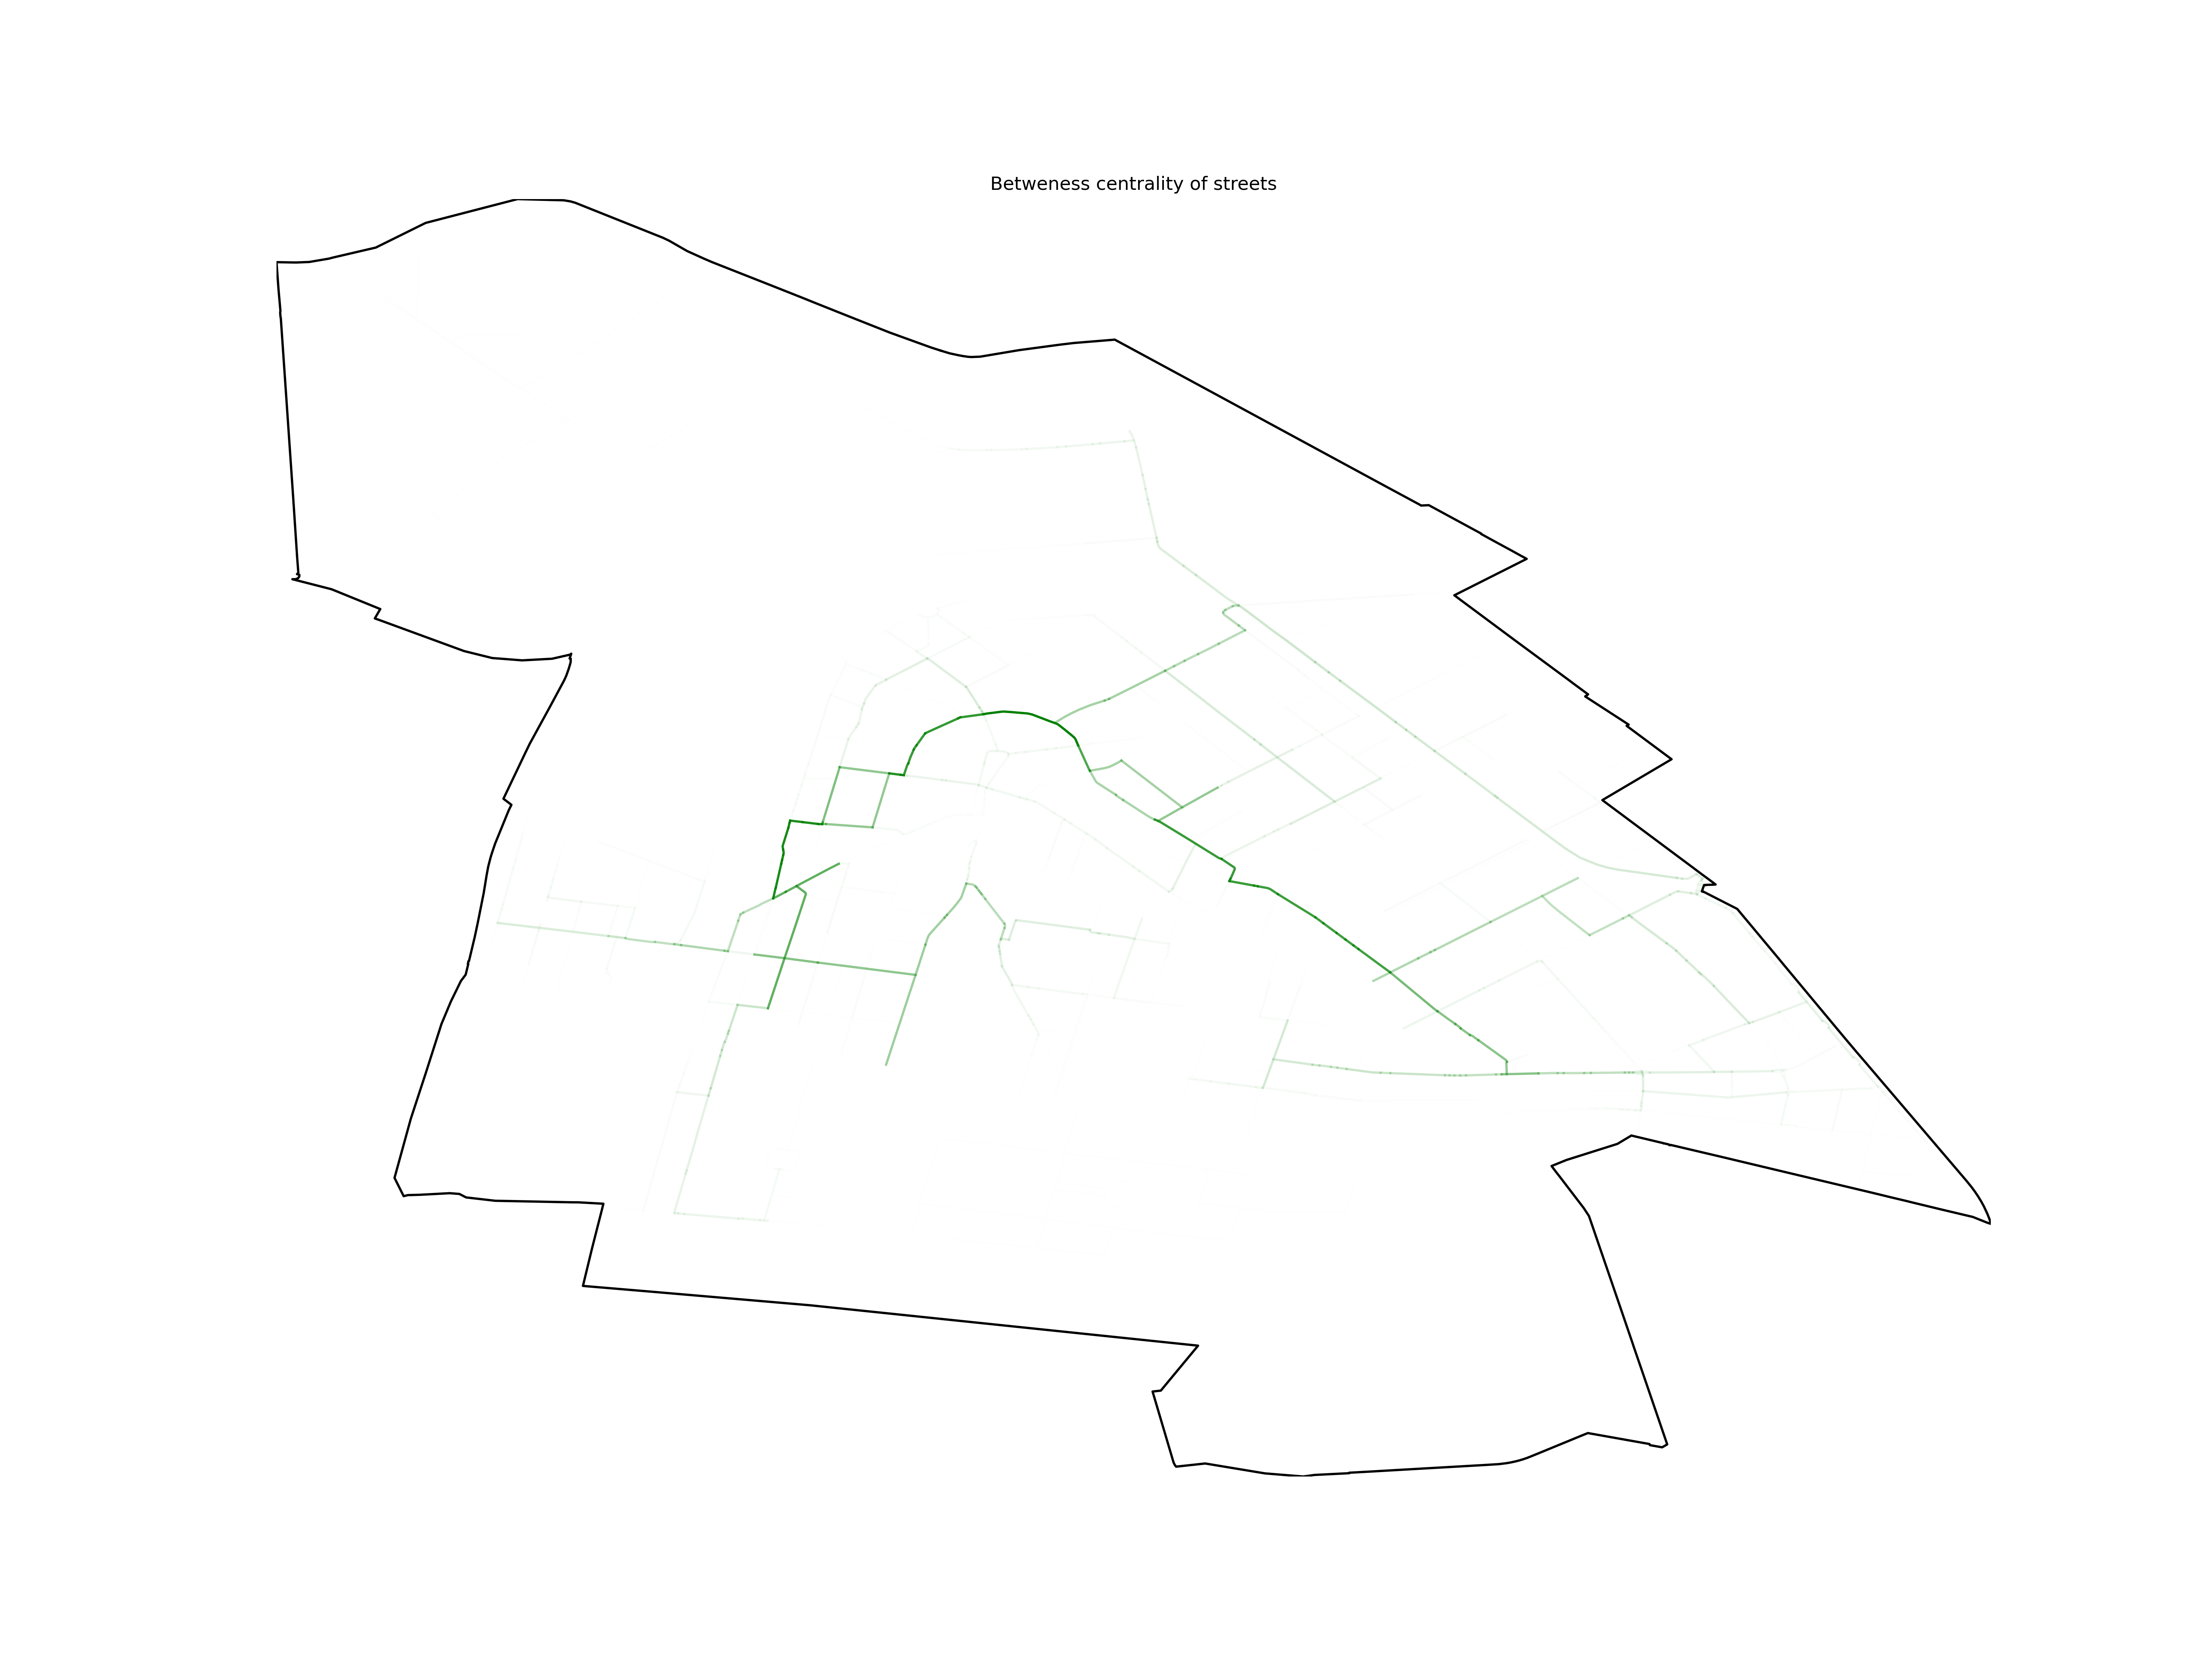
\includegraphics[width=0.5\textwidth]{figures/Adri/between.png}&  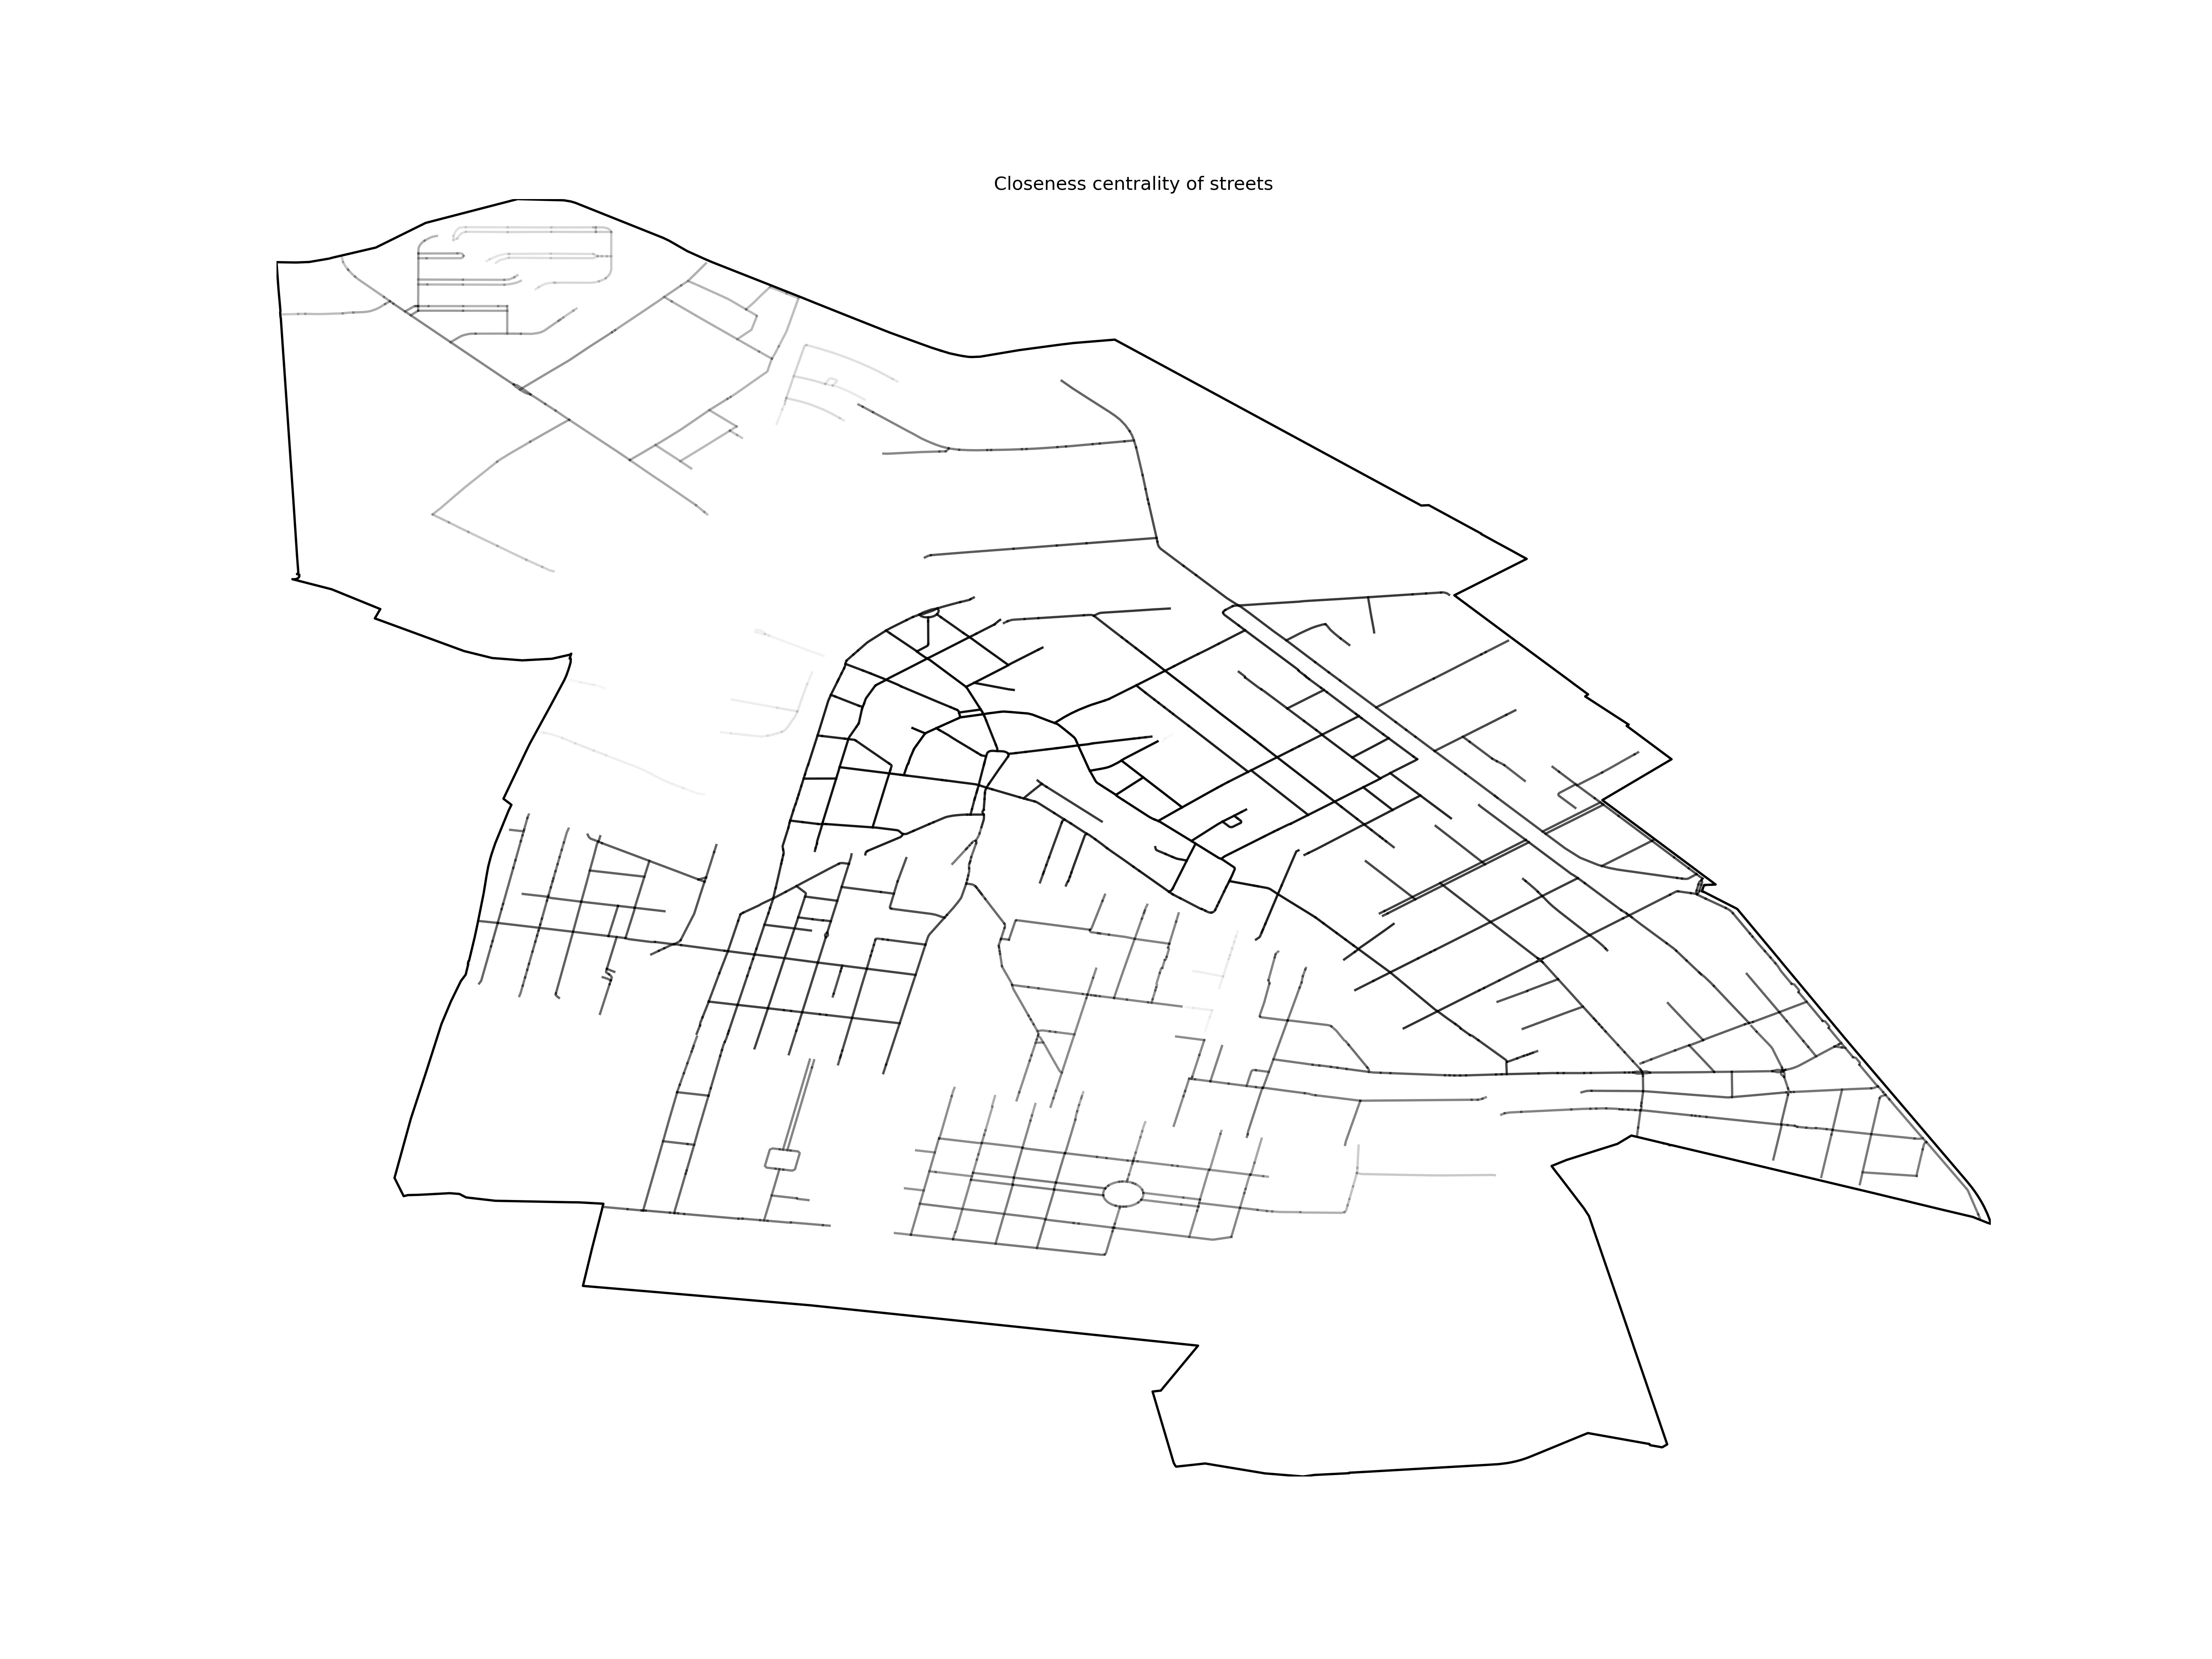
\includegraphics[width=0.5\textwidth]{figures/Adri/closeness.png}\\
         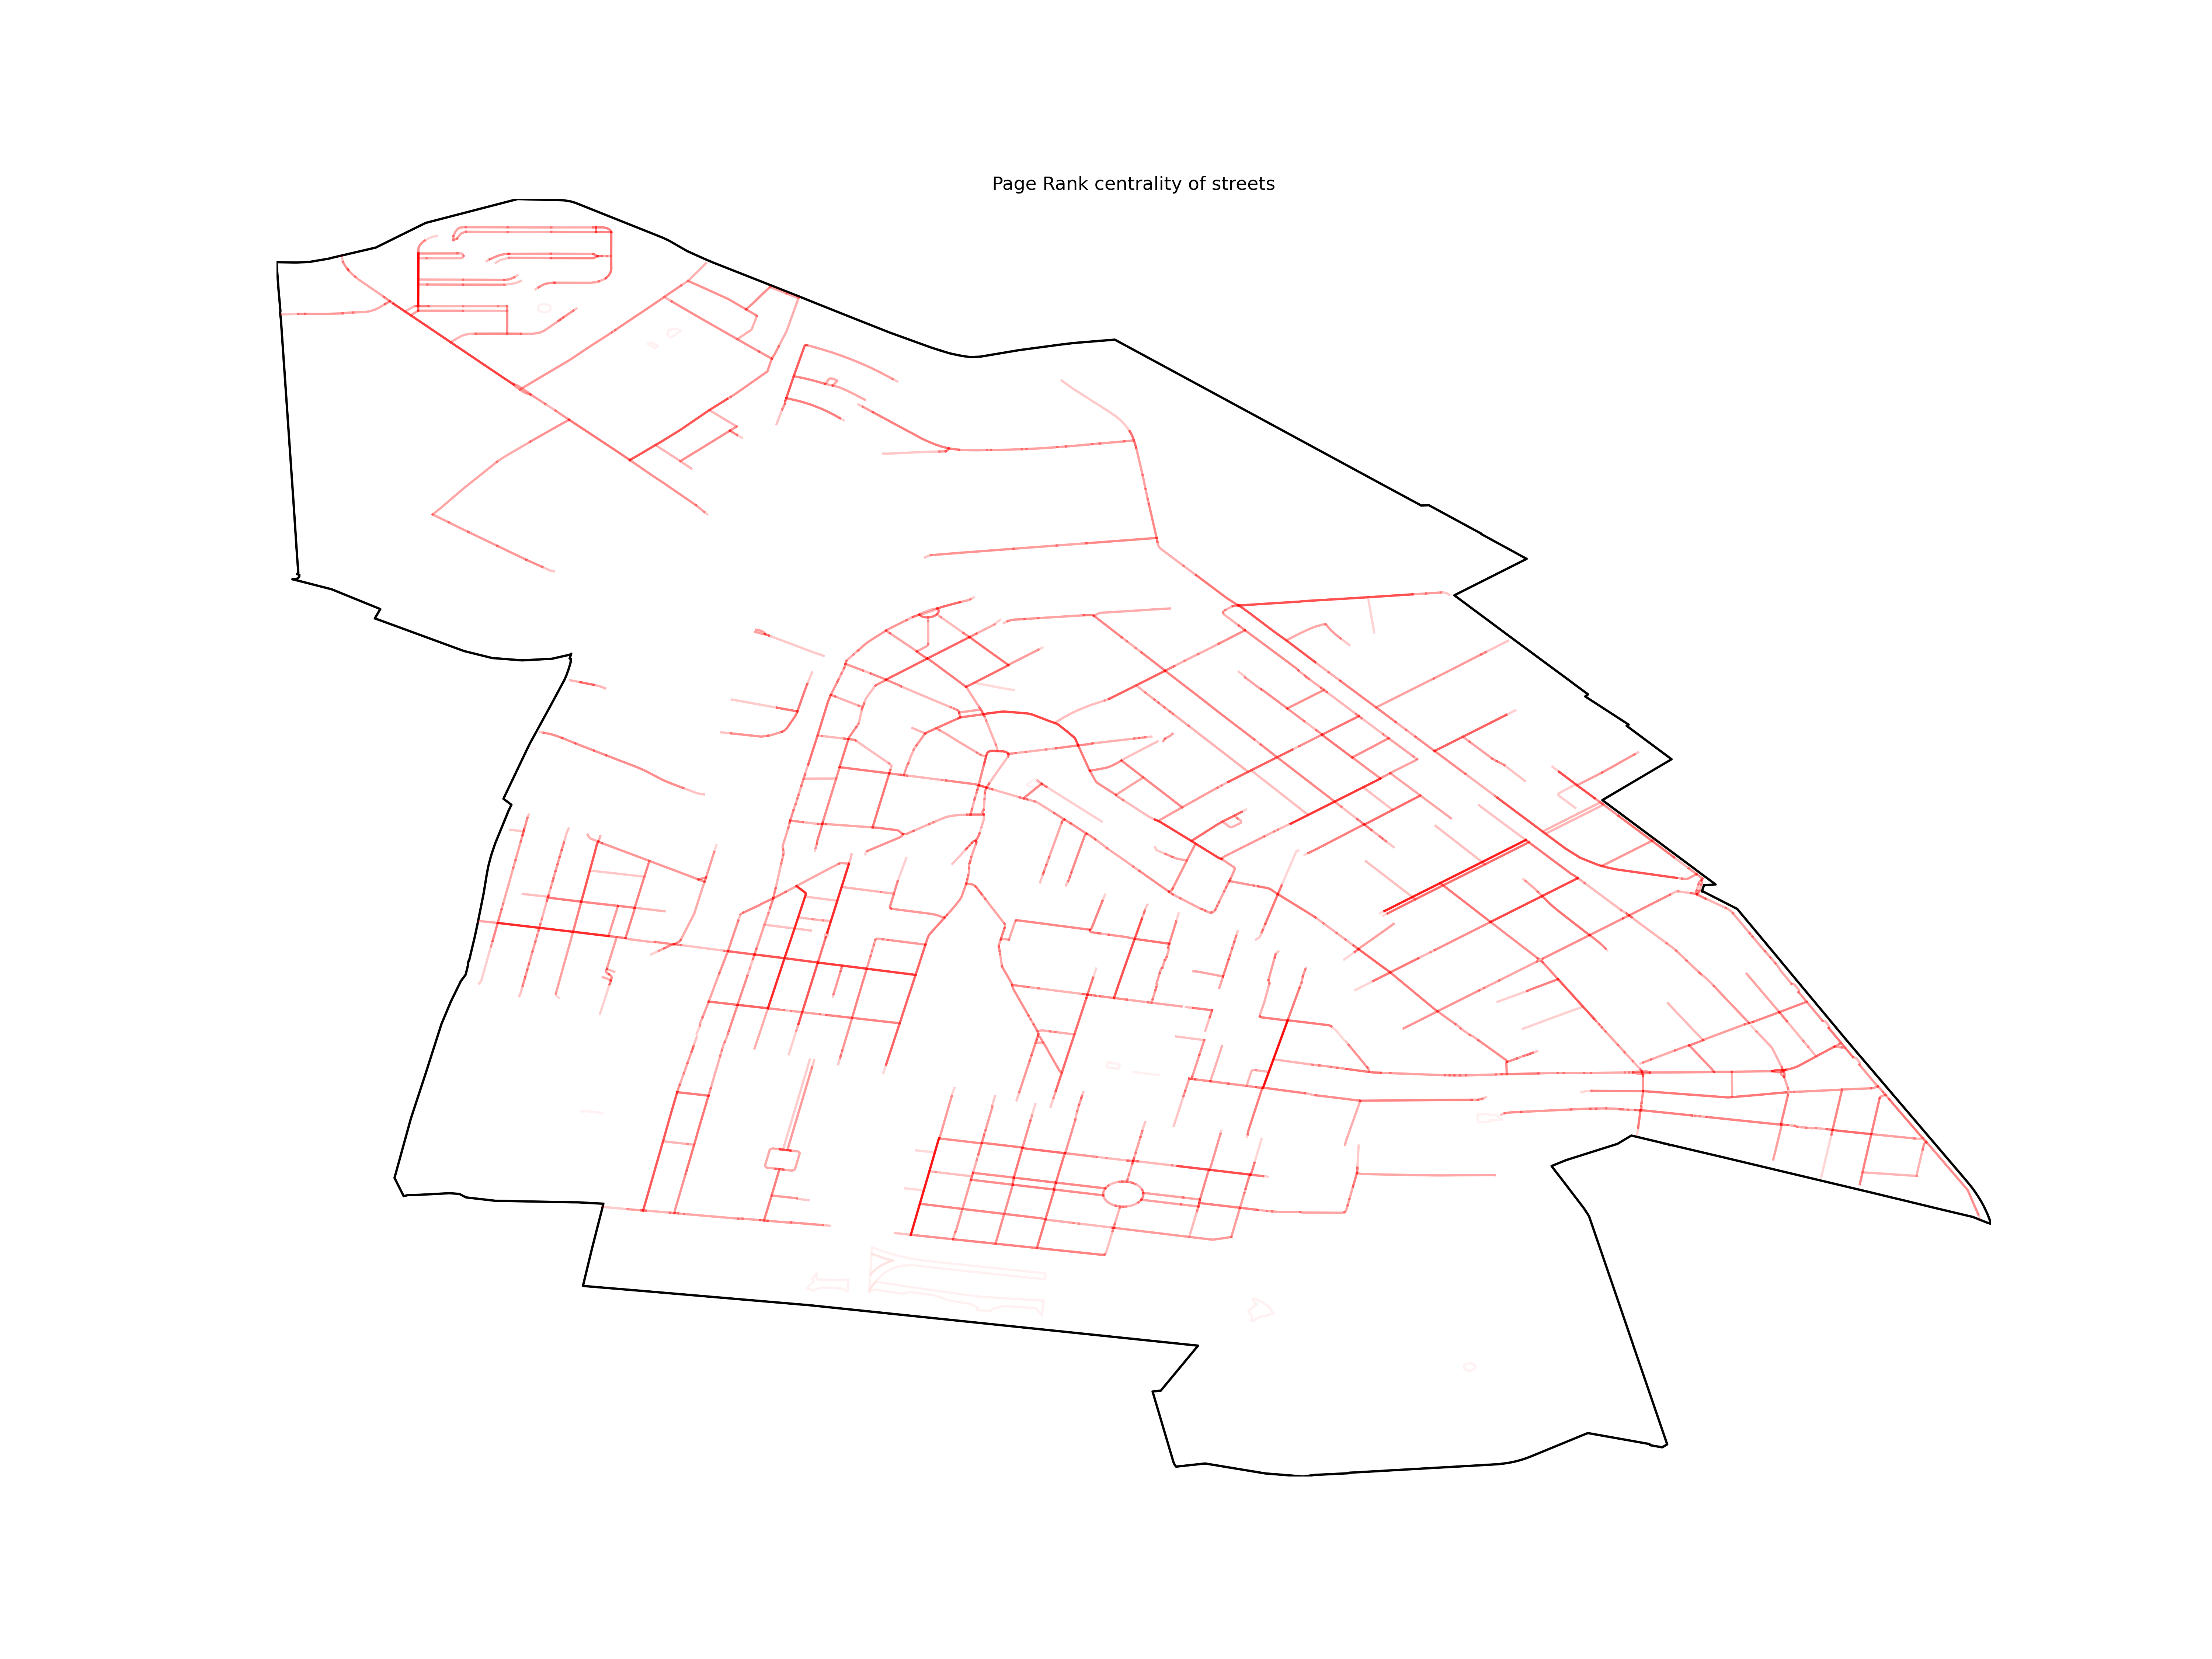
\includegraphics[width=0.5\textwidth]{figures/Adri/pagerank.png}&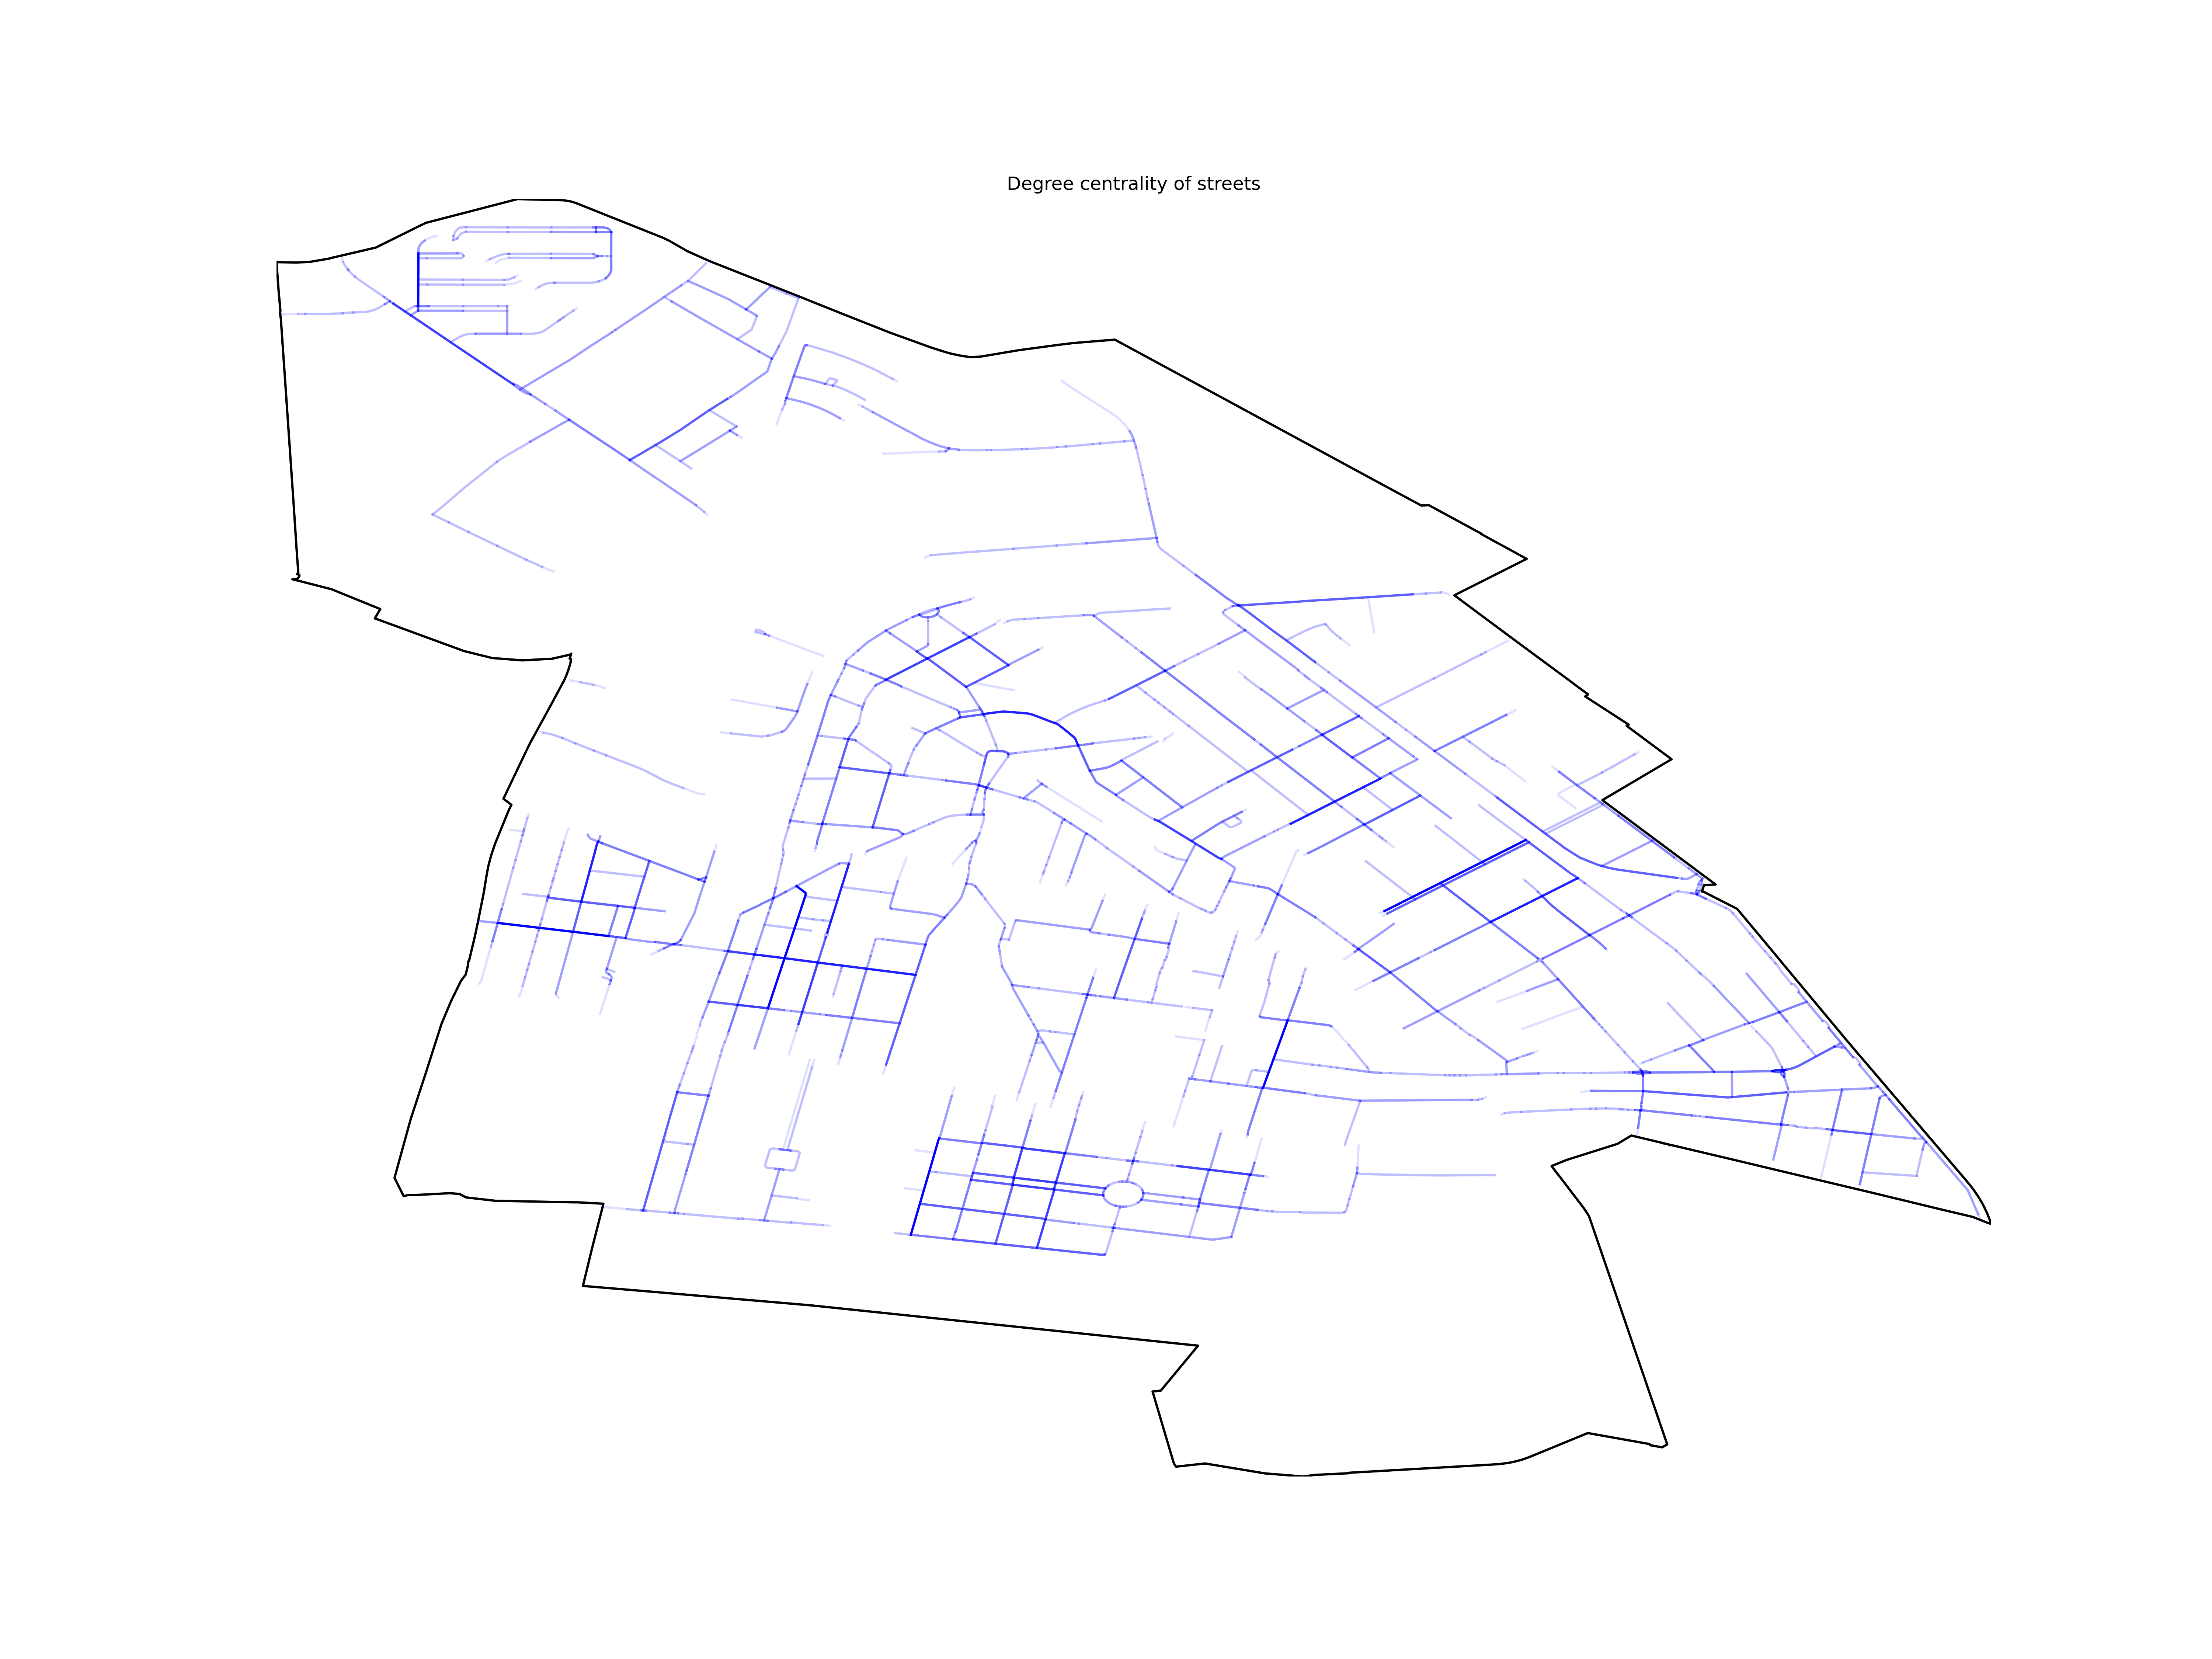
\includegraphics[width=0.5\textwidth]{figures/Adri/degree.png} 
    \end{tabular}
    \caption{Visualizations of different street centralities: Betweenness Centrality (top left), Closeness Centrality (top right), PageRank (bottom left), and Degree Centrality (bottom right). Darker regions indicate higher centrality values, providing insights into the importance and connectivity of various streets in the urban layout.}
    \label{fig:centralities}
\end{figure}

\textbf{Betweenness Centrality} measures the extent to which a street lies on the shortest path between other streets, indicating its role as a critical connector or thoroughfare. Streets with high betweenness centrality are often crucial for traffic flow, and identifying them can help in understanding and mitigating potential congestion points.

\textbf{Closeness Centrality} assesses how quickly a street can be accessed from all other streets in the network, reflecting its overall accessibility. High closeness centrality values highlight streets that are centrally located within the city's layout, making them potentially valuable for emergency response routes and efficient transportation planning.

\textbf{Degree Centrality} simply counts the number of direct connections a street has to other streets, indicating its immediate connectivity. Streets with high degree centrality are typically hubs of local activity and can be focal points for community services, commercial activities, and local traffic management.

\textbf{PageRank} centrality is inspired by the algorithm used by search engines to rank web pages, and it evaluates the influence of a street based on both its direct connections and the connections of its neighbors. Streets with high PageRank values are influential within the network, suggesting they play significant roles in the overall urban mobility and can be key targets for infrastructure improvements and urban development projects. In other work, page rank measures the portion of pedestrians that a street tends to transfer to its contiguous streets.

